\section*{Question 4}

%The deterministic finite automaton $\mathbf{M}$ is specified by checking all possible transitions. The transitions depend on the properties of $x_1$ and $x_2$ from the original processes given. For convenience, the actions shown in the original processes are listed in table \ref{tab:actions}.

The finite automaton $\mathbf{M}$ is now constructed. For convenience, the actions shown in the original processes are listed in table \ref{tab:actions}.

\begin{table}[H]
    \centering
    \begin{tabular}{cl}
    
    $a_1$:   &   $x_1 := x_2 + 1$   \vspace{2 mm}\\
    $b_1$:   &   $x_1 < x_2 \vee x_2 == 0$ \vspace{2 mm}\\
    $c_1$:   &   $x_1 := 0 $ \vspace{2 mm}\\
    $a_2$:   &   $x_2 := x_1 + 1$ \vspace{2 mm}\\
    $b_2$:   &   $x_2 < x_1 \vee x_1 == 0 $ \vspace{2 mm}\\
    $c_2$:   &   $x_2 := 0$ \\ 
    \end{tabular}
    \caption{Actions in processes. Special symbols meaning: "$:=$" assign value, "$==$" test equality.}
    \label{tab:actions}
\end{table}


The states of $\mathbf{M}$ define the the relation of properties between $x_1$ and $x_2$, and edges define possible actions. Table \ref{tab:actions} shows that $x_1$ and $x_2$ only store the same value in the special case of $x_1 = x_2 = 0$. This state is set as the initial state, since the variables start with these values. All states are seen in table \ref{tab:Mstates}. 


\begin{table}[H]
    \centering
    \begin{tabular}{cl}
    $p_0$:   &   $x_1 == 0 \land x_2 == 0$   \vspace{2 mm}\\
    $p_1$:   &   $x_1 > x_2 \land x_2 == 0$ \vspace{2 mm}\\
    $p_2$:   &   $x_1 < x_2 \land x_1 == 0 $ \vspace{2 mm}\\
    $p_3$:   &   $x_1 > x_2$ \vspace{2 mm}\\
    $p_4$:   &   $x_1 < x_2$ \\
    \end{tabular}
    \caption{States for $\mathbf{M}$ composed of variable properties (without the dead state). Possible relations are: 1) both zero \{$p_0$\}, 2) one is zero and other is positive \{$p_1$,  $p_2$\} and 3) one is larger than the other \{$p_3$, $p_4$\}.  }
    \label{tab:Mstates}
\end{table}

The transition function table, describing all edges of $\mathbf{M}$, is created from each state and action. If a test ($b_1$ or $b_2$) does not evaluate to true, the automaton cannot accept the string. Similar to the construction of $\mathbf{T}$, this is implemented with a dead state $D$. The complete transition function table is seen on table \ref{tab:Mt}.

\begin{table}[H]
    \centering
    \begin{tabular}{|c||c|c|c|c|c|c|}
    \hline
    $\delta_{\mathbf{M}}$   &   $a_1$   &   $b_1$   &   $c_1$   &   $a_2$   &   $b_2$   &   $c_2$   \\  \hline \hline
    $D$ &   $D$ &   $D$ &   $D$ &   $D$ &   $D$ &   $D$ \\ \hline
    $\rightarrow *p_0$   &   $p_1$   &   $p_0$   &   $p_0$   &   $p_2$   &   $p_0$   &   $p_0$   \\  \hline
    $*p_1$   &   $p_1$   &   $p_1$   &   $p_0$   &   $p_4$   &   $p_1$   &   $p_1$   \\  \hline   
    $*p_2$   &   $p_3$   &   $p_2$   &   $p_2$   &   $p_2$   &   $p_2$   &   $p_0$   \\  \hline
    $*p_3$   &   $p_3$   &   $D$   &   $p_2$   &   $p_4$   &   $p_3$   &   $p_1$   \\  \hline
    $*p_4$   &   $p_3$   &   $p_4$   &   $p_2$   &   $p_4$   &   $D$   &   $p_1$   \\  \hline
    \end{tabular}
    \caption{Transition function table for $\mathbf{M}$.}
    \label{tab:Mt}
\end{table}
 The final state machine is constructed from the transition function, and can be seen in figure \ref{fig:M}.

\begin{figure}[H]
    \begin{center}    
        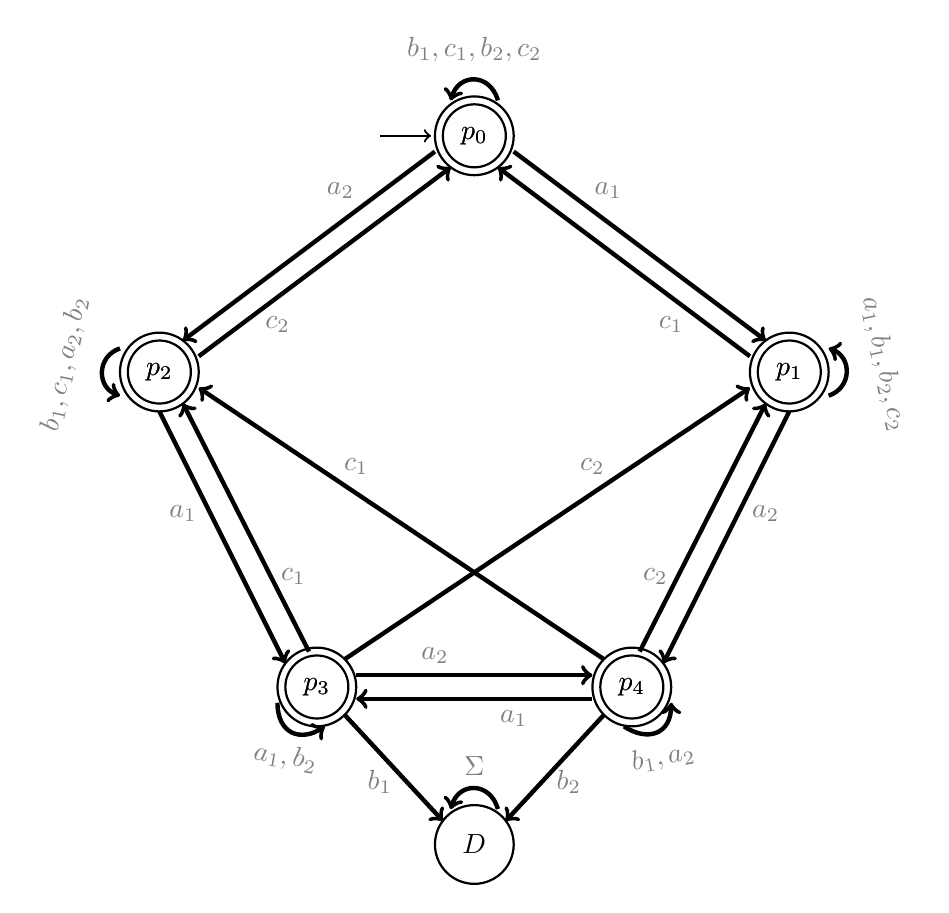
\begin{tikzpicture}
            
            %States
            \draw[thick, ->] (-1.2, 3) -- (-0.55, 3);
            \draw[thick] (0,3) circle (0.5) node {$p_0$};
            \draw[thick] (0,3) circle (0.4) node {$p_0$};
            \draw[thick] (4, 0) circle (0.5) node {$p_1$};
            \draw[thick] (4, 0) circle (0.4) node {$p_1$};
            \draw[thick] (-4, 0) circle (0.5) node {$p_2$};
            \draw[thick] (-4, 0) circle (0.4) node {$p_2$};
            \draw[thick] (-2, -4) circle (0.5) node {$p_3$};
            \draw[thick] (-2, -4) circle (0.4) node {$p_3$};
            \draw[thick] (2, -4) circle (0.5) node {$p_4$};
            \draw[thick] (2, -4) circle (0.4) node {$p_4$};
            \draw[thick] (0, -6) circle (0.5) node {$D$};
            
            %Edges
                %Normal between states
            \draw[ultra thick, ->] (0.5, 2.8) -- (3.7, 0.4);
            \draw[ultra thick, <-] (0.3, 2.6) -- (3.5, 0.2);
            
            \draw[ultra thick, ->] (-0.5, 2.8) -- (-3.7, 0.4);
            \draw[ultra thick, <-] (-0.3, 2.6) -- (-3.5, 0.2);
            
            \draw[ultra thick, ->] (4, -0.5) -- (2.4, -3.7);
            \draw[ultra thick, <-] (3.7, -0.4) -- (2.1, -3.55);
            
            \draw[ultra thick, ->] (-4, -0.5) -- (-2.4, -3.7);
            \draw[ultra thick, <-] (-3.7, -0.4) -- (-2.1, -3.55);
            
            \draw[ultra thick, ->] (-1.5, -3.85) -- (1.5, -3.85);
            \draw[ultra thick, <-] (-1.5, -4.15) -- (1.5, -4.15);
            
            \draw[ultra thick, ->] (-1.65, -4.35) -- (-0.4, -5.7);
            \draw[ultra thick, ->] (1.65, -4.35) -- (0.4, -5.7);
            
                %Diagonal across figure
            \draw[ultra thick, ->] (-1.65, -3.65) -- (3.5, -0.2);
            \draw[ultra thick, ->] (1.65, -3.65) -- (-3.5, -0.2);
            
                %%From state to same state
            \draw[ultra thick, ->] (0.3, 3.45) .. controls (0.2, 3.8) and (-0.2, 3.8) .. (-0.3, 3.45);
            \draw[ultra thick, ->] (4.5, -0.3) .. controls (4.8, -0.2) and (4.8, 0.2) .. (4.5, 0.3);
            \draw[ultra thick, <-] (-4.5, -0.3) .. controls (-4.8, -0.2) and (-4.8, 0.2) .. (-4.5, 0.3);
            \draw[ultra thick, ->] (1.9, -4.5) .. controls (2.2, -4.7) and (2.5, -4.6) .. (2.5, -4.2);
            \draw[ultra thick, <-] (-1.9, -4.5) .. controls (-2.2, -4.7) and (-2.5, -4.6) .. (-2.5, -4.2);
            \draw[ultra thick, ->] (0.3, -5.55) .. controls (0.2, -5.2) and (-0.2, -5.2) .. (-0.3, -5.55);
            
            %Labels
                %From state to other state
            \draw[gray] (1.7, 2.3) node{$a_1$};
            \draw[gray] (-1.7, 2.3) node{$a_2$};
            
            \draw[gray] (2.5, 0.6) node{$c_1$};
            \draw[gray] (-2.5, 0.6) node{$c_2$};
            
            \draw[gray] (3.7, -1.8) node{$a_2$};
            \draw[gray] (-3.7, -1.8) node{$a_1$};
            
            \draw[gray] (2.3, -2.6) node{$c_2$};
            \draw[gray] (-2.3, -2.6) node{$c_1$};
            
            \draw[gray] (0.5, -4.4) node {$a_1$};
            \draw[gray] (-0.5, -3.6) node {$a_2$};
            
            \draw[gray] (1.5, -1.2) node{$c_2$};
            \draw[gray] (-1.5, -1.2) node{$c_1$};
            
            \draw[gray] (1.2, -5.2) node{$b_2$};
            \draw[gray] (-1.2, -5.2) node{$b_1$};
            
                %From state to same state
            
            \draw[gray] (0, 4.1) node {$b_1, c_1, b_2, c_2$};
            \draw[gray] (5.2, 0.1) node[rotate = -78] {$a_1, b_1, b_2, c_2$};
            \draw[gray] (-5.2, 0.1) node[rotate = 78] {$b_1, c_1, a_2, b_2$};
            \draw[gray] (2.4, -4.9) node[rotate = 10] {$b_1, a_2$};
            \draw[gray] (-2.4, -4.9) node[rotate = -10] {$a_1, b_2$};
            \draw[gray] (0, -5) node {$\Sigma$};
            
            
        \end{tikzpicture}
    \end{center}
    \caption{Final state machine for $\mathbf{M}$. Combined with table \ref{tab:Mstates} the following state pattern can be noted. Top: Both variables are equal with a value of zero. Top middle: One of the variables is nonzero, the other is zero. Bottom middle: Both variables are non zero, but different values.  Bottom: Dead state (a test did not match current properties).}
    \label{fig:M}
\end{figure}


The final states for $\mathbf{M}$ are all states where the properties of the variables has not failed a test. The state where this is not the case, is if a test has evaluated to false. A test evaluating to false is equivalent to a processes trying to access the critical section without permission. Since this automaton's purpose is to validate the properties of the variables, it only accepts strings which does not attempt to access the critical section without permission. 

One could argue that $p_0$ should not be a final state, since neither of the two processes are able to be in the critical state at this point. But since the main goal is to validate the Bakers Algorithm and keep the two processes from entering the critical state at the same time, it seems appropriate to accept a string which ends with both processes in their initial states. 